\myparagraph{GUI}

Da brugergrænsefladen skulle laves, var der ingen tvivl om hvilket program der skulle anvendes til udarbejdelse af brugergrænsefladen. Programmet QT blev valgt da der tidligere har været arbejdet med QT i forbindelse med andre semesterprojekter. QT er et program som giver en masse muligheder som kan udnyttes. For eksempel giver QT en drag and drop mulighed, således at brugergrænsefladens udseende kan designes på en meget let og brugervenlig måde.
Sproget som brugergrænsefladen er skrevet i er C++ da det er dette sprog som teamet har haft størst erfaring med.

For at kommunikere med SPI driveren som ligger på Devkit8000 er funktionerne fread() og fwrite() brugt. Et eksempel på hvordan funktionen fwrite() blev brugt kan ses på figur x.

\begin{figure}[H]
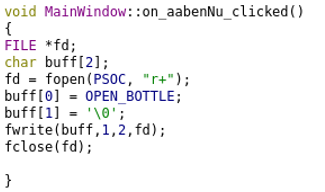
\includegraphics[scale=1]{tex/Implementering/GUI/GUI-implementering/Billeder/kodeeksempel.png}
\caption{Åben nu funktionen implementerets}
\end{figure}

På figuren ses det hvordan funktionen for trykknappen ”Åbn nu” er implementeret. PSOC er tidligere i koden blevet defineret som path’en på PSoC driven. I koden kan man se at OPEN-BOTTLE, skrives til PSoC driveren ved hjælp af fwrite(). OPEN-BOTTLE er tidligere blevet defineret som 5, hvilket i SPI protokollen betyder at vinen skal åbnes. Det er samme kode der bruges til funktionen ”Planlæg åbning”.
For at få tiden talt ned og samtidigt displayet på skærmen er der blevet benyttet threads. Implementeringen af dette kan ses i dokumentationsbilaget x.
